\section{Literature Review}\label{cha:litreview}
This chapter provides an overview of findings of literature research on the topic of (re-)entry vehicles. Firstly, past solutions and their development have been investigated for the dual purpose of reference material to be used for preliminary sizing and design and the acquisition of knowledge on mission level. Secondly, each of the primary disciplines involved in the design of a re-entry mission is investigated, namely structural design, \gls{tps}, aerodynamical design, orbital mechanics, atmospheric modelling and control. These disciplines are investigated in terms of their application and new technologies (e.g. the materials typically used for thermal protection) as well as for methods used in their respective analysis and design (e.g. the use of \gls{fem} for structural analysis).

This chapter is structured as follows. The first section gives an overview of past re-entry vehicles; the second section gives an overview of past and ongoing investigations in the use of inflatable aeroshells; subsequent sections focus on the primary distinguishable disciplines involved.

\subsection{Overview of present and past (re-)entry vehicles}\label{cha:past missions}
This section gives an overview of (re-)entry vehicles, primarily to obtain a set of reference vehicles to aid design and sizing of the payload capsule in later stages and additionally to review solutions used in the past to perform (re-)entry for human spaceflight. At this point no structure supporting the deceleration has been chosen yet. As such only payload capsule size parameters are considered. It can be argued, based on human payload requirements, that the attached payload capsule for this mission will have similar characteristics. Table \ref{tab:refmis} displays some characteristics related to the payload capsules which can be used as indicative values \footnote{Principal values from: \\
URL: \url{http://www.nasa.gov/sites/default/files/167718main\_early\_years.pdf},  Accessed: 28 April 2015 \\ URL: \url{http://www.braeunig.us/space/} Accessed: 28 April 2015 \\ \url{URL: http://wsn.spaceflight.esa.int/docs/Factsheets/35\%20Soyuz\%20LR.pdf} Accessed: 28 April 2015 \\
URL: \url{http://www.lpi.usra.edu/lunar/constellation/orion/factsheet.pdf} Accessed: 28 April 2015}. 

\begin{table}[H]
	\caption[Reference missions for payload module sizing]{Reference missions for payload module sizing.}
		\begin{tabular}{|p{0.18\textwidth}|p{0.11\textwidth}|p{0.11\textwidth}|p{0.11\textwidth}|p{0.11\textwidth}|p{0.11\textwidth}|p{0.11\textwidth}|} % MAKE SURE THAT THE TOTAL WIDTH IS 0.95\textwidth!! (that way its exactly the textwidth.... haha) 
			\hline
			Mission 						& Apollo & 	Soyuz TMA &	Shenzhou & Gemini & Mercury & Orion \\ \hline \hline
			Period [$yr$]					&	1964-1975	& 	2010-2014&	1999-2013 &   1959-1963  & 1959-1963 & Future \\ \hline
			Reentry module mass [$kg$]  	&	5806& 	2900 &	3240 & 3402 & 1118 & 8777 \\ \hline
			Habitable volume [$m^3$]		&	6.17& 	3.5  &	6.0  & 2.55 & 1.9 & 11   \\ \hline
			Diameter [$m$]			 		&	3.9 & 	2.17  &	2.52 & 2.3 & 1.9 & 5   \\ \hline
			Length  [$m$]			 		&	3.5 & 	2.24  &	2.5  & 3.4 &  5.2 & Unknown  \\ \hline
			Crew size (max) [$persons$]		&	3   & 	3     &	3    & 2   &  1   & 6   \\ \hline
		\end{tabular}
    \label{tab:refmis}
\end{table}

It must be noted that Table \ref{tab:refmis} displays typical values only to be used as first indicative values. For example the diameter is typically a maximum value since no single value can be supplied due to the cone like shape of most reentry vehicles. Moreover these designs include the size and mass of the deceleration system of which the latter typically includes a heavy duty heat shield. Most re-entry vehicle base designs were used multiple times with minor design changes and a single externally communicated design name. As such the values in the table above should be used with proper care as indicative values only. Habitable volume estimation also depends on the mission duration and the variation thereof may be considerable. A study on the estimation of these parameters is given in Ref.\cite{Rudisill2008}. Although this study focuses on a lunar mission, it still underlines many of the important aspects with respect to payload module sizing which are applicable for Mars missions as well. It may as such prove a proper foundation for payload module sizing. 

From the reference missions in Table \ref{tab:refmis} especially the future Orion mission, currently being designed, is of great interest. The Orion crew exploration vehicle is planned to go to the Moon, Mars and further in the solar system. Being designed for similar missions distances using present day technologies the Orion mission can as such be considered as the primary reference payload.



\subsection{Review of aeroshell technology}\label{sec:aeroshells}

\subsubsection{Advantages of inflatable aeroshells}
Inflatable aeroshell systems provide the following advantages with respect to traditional rigid aeroshells: \cite{cassapakis, IRVEoverview} 
\begin{enumerate}
\item A lower weight is typically achieved, as investigated by Ref.\cite{Cruz} and to some extent Ref.\cite{EDLASphase1};
\item An unconstrained inflatable diameter, by the launch vehicle fairing, allows use of larger aerodynamic decelerators. As a result a lower \gls{bc} is achievable;
\item A smaller aeroshell volume fraction is required by a lack of need to use a backshell to protect the payload from aft side heating (in contrast to rigid aeroshells);
\item Effective cocooning of the payload by a rigid aeroshell diminishes accessibility. Adding access ports requires the use of additional verification and validation of thermal control design \cite{johnsonstardust}.
\item Heat is trapped by a rigid aeroshell cocooning the payload, causing potential interference with on-board payload thermal requirements.
\end{enumerate}
Of these reasons, the first two prevail for the current mission in view of constraints by the launch vehicle, limiting entry vehicle mass and diameter. A way of handling the diameter constraints, one in the launcher fairing shroud and a more relaxed one after decoupling of launcher and entry vehicle, is utilizing deployment mechanisms. These may be either mechanical or inflatable. Comparison of these two concepts yields the following characteristics in favour of inflatable structures \cite{cassapakis}:
\begin{enumerate}
\item Inflatables have a high reliability of deployment due to a self-correcting system;
\item Use of thin materials obtaining strength from inflation gas pressure reduces the weight required for inflatable systems compared to mechanical structures;
\item Packaging efficiency is higher for inflatable structures than for mechanical erectable structures;
\item Loads are absorbed over a large surface area for inflatable structures, as opposed to typical load concentrations in mechanical systems. Load concentrations require local addition of weight, typically resulting in a heavier structure;
\item Inflatables have a typically lower production cost;
\item Easily adapted to concave shapes with symmetric and curved surfaces;
\item Favorable dynamics due to the nearly constant inflation pressure induced force restoring encountered surface distortions;
\item A favorable thermal response by radiation exchange over a large area.
\end{enumerate}

\subsubsection{Investigation of Aeroshell Technology}
The aforementioned reasons, primarily lower weight and high packaging efficiency, have been key drivers in past and ongoing research in the use of inflatable structures for use in aerodynamic deceleration during (re-)entry. Primary contributor is \gls{nasa}, specifically NASA Langley Research Center, responsible for a series of tests on the feasibility and use of \gls{hiad} concepts for entry and re-entry \cite{irve1, irve2, irve3, thor}. A brief discussion on these tests follows.

\gls{irve} II successfully met its objectives, namely: "to demonstrate inflation and re-entry survivability, assess the thermal and drag performance of the re-entry vehicle and to collect flight data for comparison with analysis and design techniques used in vehicle development" \cite[p.1]{flightperfirve2}. IRVE-II consisted of a rigid, cylindrical centerbody with a deployable, conical inflatable aeroshell of a so-called stacked toroid configuration \cite{histoverviewtech,vehicleflexibilityirve2}.

IRVE-III proceeded with its primary aim to demonstrate the offset of the vehicle center of gravity on the lift-to-drag ratio of the vehicle, while subsystems were altered: support straps were added to inter- and intraconnect toroids and centerbody, the \gls{tps} was upgraded by a choice

\subsection{Structures in (re-)entry vehicles}\label{sec:struc}
Firstly applications and technologies, within the field of structures and materials, as applied in (re-)entry vehicles are investigated, with an emphasis on inflatable aeroshells. Secondly, methods for structural analysis and design are investigated for their effectiveness and feasibility in the project at hand.

\subsubsection{Non-inflatable structures}
Non-inflatable structures have a

\subsubsection{Inflatable structures}
Inflatable structures may be preferable to conventional non-inflatable structures for a number of structural reasons 





After the model construction verification was carried out to determine whether the model correctly implemented the calculations of the modified Newtonian method. This was done by placing two triangular surface elements in a flow. First at an angle and secondly normal to the flow. The model outputs were verified by also calculating the results by hand.

Following the verification process the model was validated using experimental values of different parameters. Each separate validation case will be treated here.

\subsubsection{\gls{sym:CD}-validation against experimental drag of a sphere}
\label{subsubsec:valsphere}
For the first model validation case a comparison was made the between the \gls{sym:CD}-value of a sphere in hypersonic flow that were computed by the model and as found in an experiment. It was found that for hypersonic Mach numbers the experimental \gls{sym:CD}-value of a sphere is $0.92$ \cite{Bailey1966,AndersonJr.2007,Cox1965}. When computing \gls{sym:CD} numerically with the modified Newtonian method using more than $10,000$ surface elements produces $\gls{sym:CD}=0.916$, which coincides with a discrepancy of $0.5\%$ of the experimental value. Since the accuracy of the experimental data is approximately $\pm1.5\%$ \cite{Bailey1966} this discrepancy falls within the confidence interval of the measurements.

\subsubsection{\gls{sym:CP}-validation against experimental data of a sharp cone}
\label{subsubsec:valsharpconeCP}
Following the \gls{sym:CD}-validation for blunt bodies presented in the previous section now \gls{sym:CP}-validation will be carried out for sharp bodies. This is performed by comparing \gls{sym:CP} at select points on the surface of a cone with half-cone angle \gls{sym:theta} of $15$ degrees. The experimental data was collected for $\gls{sym:M}=14.9$ and $\gls{sym:gamma}=\frac{5}{3}$  \cite{Bertin1994,Cleary1970}. Figure \ref{fig:CPcone30val} shows the data points that were collected for angles of attack $\gls{sym:alpha}=10[\deg]]$ and $\gls{sym:alpha}=20[\deg]$ in Figure \ref{fig:CPconealpha10} and \ref{fig:CPconealpha20} respectively. On the X-axis the variable \gls{sym:beta_cone} is used. This quantity refers to the local cross-sectional surface rotation with respect to an axis that is defined positive in the positive Z-direction. Figure \ref{fig:beta_cone} showcases this concept more clearly. Normally the domain of \gls{sym:beta_cone} lies between $0[\deg]$ and $360[\deg]$, but because the cone is symmetrical only half of the cone surface is plotted here. Furthermore, since the cone in question is a sharp cone with a constant semi-cone angle the \gls{sym:CP}-distribution is constant along the cone surface for constant \gls{sym:beta_cone}.
As can be seen in Figures \ref{fig:CPconealpha10} and \ref{fig:CPconealpha20} the modified Newtonian method is the most accurate around $\gls{sym:beta_cone}=90[\deg]$.

\begin{figure}[h]
	\centering
	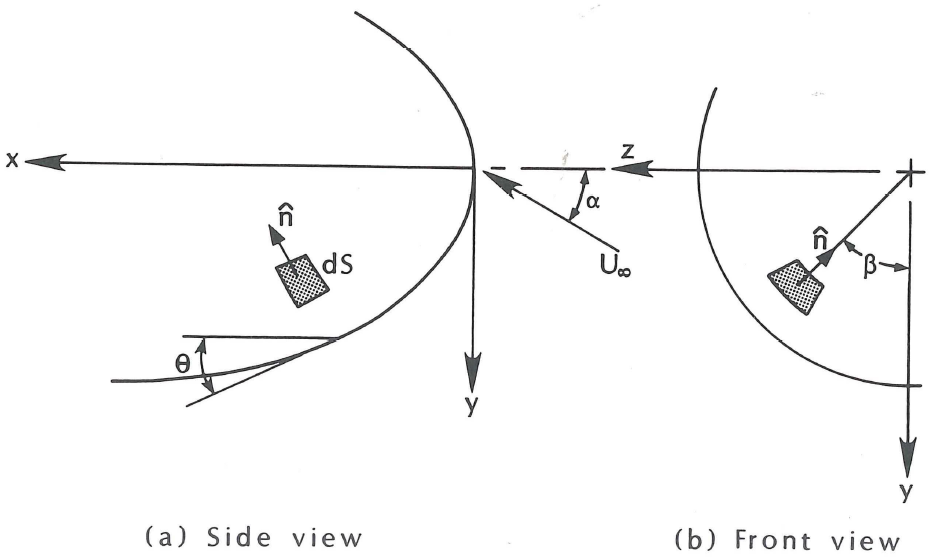
\includegraphics[width=0.7\textwidth]{./Figure/Aerodynamics/def_beta}
	\caption[Definition of \gls{sym:beta_cone}]{Definition of \gls{sym:beta_cone} \cite{Bertin1994}}
	\label{fig:beta_cone}
\end{figure}

\begin{figure}[h]
	\centering
	\begin{subfigure}[b]{0.49\textwidth}
		\centering
		\setlength\figureheight{0.6\textwidth} 
		\setlength\figurewidth{0.85\textwidth}
		% This file was created by matlab2tikz.
% Minimal pgfplots version: 1.3
%
\definecolor{mycolor1}{rgb}{0.20810,0.16630,0.52920}%
\definecolor{mycolor2}{rgb}{0.19855,0.72140,0.63095}%
%
\begin{tikzpicture}

\begin{axis}[%
width=0.95092\figurewidth,
height=\figureheight,
at={(0\figurewidth,0\figureheight)},
scale only axis,
xmin=0,
xmax=200,
xlabel={$\beta$ [deg]},
xmajorgrids,
ymin=0,
ymax=0.4,
ylabel={$C_p$ [-]},
ymajorgrids,
legend style={legend cell align=left,align=left,draw=white!15!black}
]
\addplot [color=mycolor1,solid]
  table[row sep=crcr]{%
0	0.313663919882391\\
4.55696202531646	0.312877849005529\\
9.11392405063291	0.310530499749308\\
13.6708860759494	0.306654244746176\\
18.2278481012658	0.301302318547099\\
22.7848101265823	0.29454775570286\\
27.3417721518987	0.286481939294681\\
31.8987341772152	0.277212794080603\\
36.4556962025316	0.266862666715091\\
41.0126582278481	0.255565942738302\\
45.5696202531646	0.243466456039843\\
50.126582278481	0.230714751131957\\
54.6835443037975	0.217465261705828\\
59.2405063291139	0.203873470516536\\
63.7974683544304	0.190093115610837\\
68.3544303797468	0.176273506281338\\
72.9113924050633	0.162557008944947\\
77.4683544303798	0.14907675848562\\
82.0253164556962	0.135954644591526\\
86.5822784810127	0.123299615408348\\
91.1392405063291	0.111206332607406\\
95.6962025316456	0.0997542029384269\\
100.253164556962	0.0890068017311918\\
104.810126582279	0.0790116938710017\\
109.367088607595	0.0698006477512688\\
113.924050632911	0.0613902278554033\\
118.481012658228	0.0537827421878944\\
123.037974683544	0.046967511998371\\
127.594936708861	0.0409224233429402\\
132.151898734177	0.0356157132021625\\
136.708860759494	0.0310079372951395\\
141.26582278481	0.0270540625330662\\
145.822784810127	0.023705624346723\\
150.379746835443	0.0209128879663695\\
154.93670886076	0.0186269531555022\\
159.493670886076	0.016801743887958\\
164.050632911392	0.0153958279571552\\
168.607594936709	0.0143740164247398\\
173.164556962025	0.0137086990254263\\
177.721518987342	0.0133808789844762\\
182.278481012658	0.0133808789844762\\
};
\addlegendentry{Modified Newtonian};

\addplot [color=mycolor2,only marks,mark=asterisk,mark options={solid}]
  table[row sep=crcr]{%
0	0.359\\
30	0.326\\
60	0.234\\
90	0.112\\
120	0.06\\
150	0.037\\
180	0.039\\
};
\addlegendentry{Measured};

\end{axis}
\end{tikzpicture}%
		\caption{$\gls{sym:alpha}=10\deg$}
		\label{fig:CPconealpha10}
	\end{subfigure}
		\begin{subfigure}[b]{0.49\textwidth}
			\centering
			\setlength\figureheight{0.6\textwidth} 
			\setlength\figurewidth{0.85\textwidth}
			% This file was created by matlab2tikz.
% Minimal pgfplots version: 1.3
%
\definecolor{mycolor1}{rgb}{0.20810,0.16630,0.52920}%
\definecolor{mycolor2}{rgb}{0.19855,0.72140,0.63095}%
%
\begin{tikzpicture}

\begin{axis}[%
width=0.95092\figurewidth,
height=\figureheight,
at={(0\figurewidth,0\figureheight)},
scale only axis,
xmin=0,
xmax=200,
xlabel={$\beta$ [deg]},
xmajorgrids,
ymin=0,
ymax=0.7,
ylabel={$C_p$ [-]},
ymajorgrids,
legend style={legend cell align=left,align=left,draw=white!15!black}
]
\addplot [color=mycolor1,solid]
  table[row sep=crcr]{%
0	0.577764228354504\\
4.55696202531646	0.575664128443356\\
9.11392405063291	0.569399969689605\\
13.6708860759494	0.559079369250394\\
18.2278481012658	0.544879022785013\\
22.7848101265823	0.527040773405377\\
27.3417721518987	0.505866243155278\\
31.8987341772152	0.481710157904938\\
36.4556962025316	0.454972528255649\\
41.0126582278481	0.426089876689746\\
45.5696202531646	0.395525724083726\\
50.126582278481	0.363760566256924\\
54.6835443037975	0.331281583018694\\
59.2405063291139	0.298572327912705\\
63.7974683544304	0.26610264639941\\
68.3544303797468	0.234319063584449\\
72.9113924050633	0.203635869964691\\
77.4683544303798	0.174427115348786\\
82.0253164556962	0.1470196975823\\
86.5822784810127	0.121687704566509\\
91.1392405063291	0.0986481360184979\\
95.6962025316456	0.0780580962897468\\
100.253164556962	0.0600135122299421\\
104.810126582279	0.044549391495899\\
109.367088607595	0.0316415978371448\\
113.924050632911	0.0212100817210665\\
118.481012658228	0.0131234681544689\\
123.037974683544	0.00720486963515046\\
127.594936708861	0.00323876168105333\\
132.151898734177	0.000978732102579191\\
136.708860759494	0.000121379574901702\\
141.26582278481	0\\
145.822784810127	0\\
150.379746835443	0\\
154.93670886076	0\\
159.493670886076	0\\
164.050632911392	0\\
168.607594936709	0\\
173.164556962025	0\\
177.721518987342	0\\
182.278481012658	0\\
};
\addlegendentry{Modified Newtonian};

\addplot [color=mycolor2,only marks,mark=asterisk,mark options={solid}]
  table[row sep=crcr]{%
0	0.63\\
30	0.55\\
60	0.327\\
90	0.093\\
120	0.028\\
150	0.009\\
180	0.014\\
};
\addlegendentry{Measured};

\end{axis}
\end{tikzpicture}%
		\caption{$\gls{sym:alpha}=20\deg$}
		\label{fig:CPconealpha20}
	\end{subfigure}
	\caption{Comparisons between experimental and numerical pressure coefficients}
	\label{fig:CPcone30val}
\end{figure}

\subsubsection{\gls{sym:CD}-validation against experimental data of a sharp cone}
\label{subsubsec:valsharpconeCD}
Stevens found that for a sharp cone-cylinder with half-cone angle \gls{sym:theta} of $30\deg$ $\gls{sym:CD}=0.58$ in an air-stream of Mach $8$ where angle of attack \gls{sym:alpha} and sideslip angle \gls{sym:beta} are zero \cite{Stevens1950,AndersonJr.2007}. The numerical model predicts for this case that $\gls{sym:CD}=0.456$, which coincides with a discrepancy of $21.4\%$ of the experimental value. This is in line with the results of section \ref{subsubsec:valsharpconeCP} where the \glspl{sym:CP} predicted by the numerical model were smaller than the experimental values of a sharp cone.

\subsubsection{\gls{sym:CP}-validation against experimental data of the Apollo re-entry capsule}
\label{subsubsec:Apollo_validation}
The data points in Figure \ref{fig:Apollo_cp} represent pressure coefficients measured at various locations of one of the two axisymmetric axes \cite{Bertin1966}. The quantity shown on the X-axis is defined in Figure \ref{fig:Apollo_y}. As can be seen in Figure \ref{fig:Apollo_cp} the numerical model is most accurate around the centre of the capsule. As the distance to the centreline increases, so does the discrepancy between the experimental and numerical values.

\begin{figure}[H]
	\centering
	\setlength\figureheight{0.4\textwidth} 
	\setlength\figurewidth{0.95\textwidth}
	% This file was created by matlab2tikz.
% Minimal pgfplots version: 1.3
%
\definecolor{mycolor1}{rgb}{0.20810,0.16630,0.52920}%
\definecolor{mycolor2}{rgb}{0.19855,0.72140,0.63095}%
%
\begin{tikzpicture}

\begin{axis}[%
width=0.95092\figurewidth,
height=\figureheight,
at={(0\figurewidth,0\figureheight)},
scale only axis,
unbounded coords=jump,
xmin=-1.5,
xmax=1.5,
xlabel={$\frac{s}{R}$ [-]},
xmajorgrids,
ymin=0,
ymax=1.8,
ylabel={$C_p$ [-]},
ymajorgrids,
legend style={at={(0.5,0.03)},anchor=south,legend cell align=left,align=left,draw=white!15!black}
]
\addplot [color=mycolor1,solid]
  table[row sep=crcr]{%
-1.095	0.00194223338446491\\
-1.09496992147514	0\\
-1.09472939221993	0.0105764109659139\\
-1.09463923908848	0\\
-1.09415883985204	0.0286612804702033\\
-1.09400885921748	0\\
-1.09328990674072	0.0560242775566994\\
-1.09308050968954	0\\
-1.09212497457122	0.092367937353207\\
-1.09185673504618	0\\
-1.09066723634165	0.137297047773714\\
-1.09034088956864	0\\
-1.08892068761116	0.190322850013229\\
-1.08853712808401	0\\
-1.08689011554844	0.250868241388263\\
-1.08645039457714	nan\\
-1.08458108581034	0.318273930108563\\
-1.0819999272869	0.3918054818373\\
-1.07915371475421	0.470661188513422\\
-1.07605024948299	0.55398068095838\\
-1.07269803785581	0.640854198362098\\
-1.06910626805175	0.730332419944821\\
-1.06528478486218	0.821436757031353\\
-1.06124406270688	0.913169997566455\\
-1.05699517692443	1.00452718986455\\
-1.05254977341541	1.09450664823589\\
-1.04792003672184	1.18212096017887\\
-1.0431186566302	1.26640787317747\\
-1.03815879338958	1.34644093888065\\
-1.03305404164036	1.42133979364298\\
-1.02781839315226	1.42835417521564\\
-1.01832656548985	1.44935521736688\\
-0.986104624404206	1.50751538767456\\
-0.953709183690762	1.52351962805163\\
-0.921145943147255	1.5390688207566\\
-0.888420632094868	1.55415195599687\\
-0.855539008370191	1.56875835245074\\
-0.822506857312158	1.58287766497233\\
-0.789329990744154	1.59649989205813\\
-0.75601424595145	1.60961538306931\\
-0.72256548465417	1.62221484520418\\
-0.688989591975953	1.63428935021542\\
-0.655292475408497	1.64583034086682\\
-0.621480063772172	1.6568296371244\\
-0.587558306172872	1.66727944207735\\
-0.553533170955306	1.67717234758383\\
-0.519410644652901	1.68650133963741\\
-0.485196730934503	1.69525980344988\\
-0.450897449548067	1.7034415282464\\
-0.416518835261513	1.71104071176934\\
-0.382066936800948	1.71805196448708\\
-0.347547815786417	1.72447031350459\\
-0.312967545665402	1.7302912061727\\
-0.27833221064423	1.73551051339311\\
-0.243647904617593	1.74012453261658\\
-0.208920730096357	1.74412999053202\\
-0.174156797133862	1.74752404544416\\
-0.139362222250891	1.7503042893381\\
-0.104543127359504	1.75246874962895\\
-0.0697056386859186	1.75401589059533\\
-0.0348558856926369	1.75488268492153\\
-0	1.75525426236477\\
0.0348558856926369	1.75488268492153\\
0.0697056386859186	1.75401589059533\\
0.104543127359504	1.75246874962895\\
0.139362222250891	1.7503042893381\\
0.174156797133862	1.74752404544416\\
0.208920730096357	1.74412999053202\\
0.243647904617593	1.74012453261658\\
0.27833221064423	1.73551051339311\\
0.312967545665402	1.7302912061727\\
0.347547815786417	1.72447031350459\\
0.382066936800948	1.71805196448708\\
0.416518835261513	1.71104071176934\\
0.450897449548067	1.7034415282464\\
0.485196730934503	1.69525980344988\\
0.519410644652901	1.68650133963741\\
0.553533170955306	1.67717234758383\\
0.587558306172872	1.66727944207735\\
0.621480063772172	1.6568296371244\\
0.655292475408497	1.64583034086682\\
0.688989591975953	1.63428935021542\\
0.72256548465417	1.62221484520418\\
0.75601424595145	1.60961538306931\\
0.789329990744154	1.59649989205813\\
0.822506857312158	1.58287766497233\\
0.855539008370191	1.56875835245074\\
0.888420632094868	1.55415195599687\\
0.921145943147255	1.5390688207566\\
0.953709183690762	1.52351962805163\\
0.986104624404206	1.50751538767456\\
1.01832656548985	1.44935521736688\\
1.02781839315226	1.42835417521564\\
1.03305404164036	1.42133979364298\\
1.03815879338958	1.34644093888065\\
1.0431186566302	1.26640787317747\\
1.04792003672184	1.18212096017886\\
1.05254977341541	1.09450664823589\\
1.05699517692443	1.00452718986455\\
1.06124406270688	0.913169997566455\\
1.06528478486218	0.821436757031353\\
1.06910626805175	0.730332419944821\\
1.07269803785581	0.640854198362098\\
1.07605024948299	0.55398068095838\\
1.07915371475421	0.470661188513422\\
1.0819999272869	0.3918054818373\\
1.08458108581034	0.318273930108563\\
1.08645039457714	nan\\
1.08689011554844	0.250868241388263\\
1.08853712808401	0\\
1.08892068761116	0.190322850013229\\
1.09034088956864	0\\
1.09066723634165	0.137297047773714\\
1.09185673504618	0\\
1.09212497457122	0.0923679373532069\\
1.09308050968954	0\\
1.09328990674072	0.0560242775566994\\
1.09400885921748	0\\
1.09415883985204	0.0286612804702033\\
1.09463923908848	0\\
1.09472939221993	0.0105764109659139\\
1.09496992147514	0\\
1.095	0.0019422333844649\\
};
\addlegendentry{Modified Newtonian};

\addplot [color=mycolor2,only marks,mark=asterisk,mark options={solid}]
  table[row sep=crcr]{%
-1.02718093698553	0.326751322056051\\
-0.951551131339198	1.02168543257076\\
-0.799264139197169	1.4880212545932\\
-0.247616441864002	1.7300201625693\\
0.0180691662280614	1.74873159897289\\
0.273850147488554	1.70299372722051\\
0.547682381293604	1.63105638244619\\
0.68183629061674	1.49350323432687\\
0.817930550476365	1.44043342939967\\
0.871460439771112	1.37207156639853\\
0.929404854806911	1.26182928317321\\
0.981710021888355	0.939565894363321\\
1.0408671541418	0.31807000221393\\
1.09530512997895	0.0391870122023066\\
};
\addlegendentry{Measured};

\end{axis}
\end{tikzpicture}%
	\caption{Comparison between experimental and numerical \glspl{sym:CP} for the Apollo re-entry capsule}
	\label{fig:Apollo_cp}
\end{figure}

\begin{figure}[H]
	\centering
	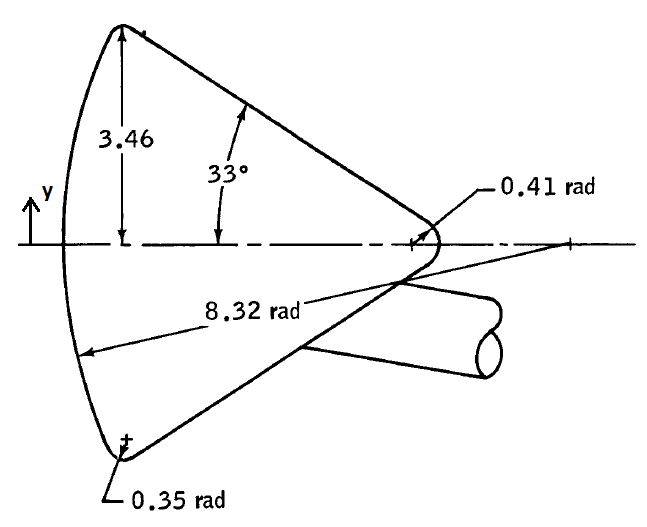
\includegraphics[width=0.4\textwidth]{./Figure/Aerodynamics/Apollo_model}
	\caption[Definition of unit on the horizontal axis of Figure \ref{fig:Apollo_cp}]{Definition of unit on the horizontal axis of Figure \ref{fig:Apollo_cp} \cite{Bertin1966}}
	\label{fig:Apollo_y}
\end{figure}

\subsubsection{Maximum heat flux validation against experimental data of the \gls{irve} 3 vehicle}
\label{subsubsec:heatvalidation}
Dillman et al. observed that the maximum heat flux on the \acrfull{irve} 3 was $14.4$ $[W\cdot cm^{-2}]$ during re-entry at an altitude of $50$ kilometres and Mach $7.0$ \cite{Dillman2012}. The maximum heat flux computed by the numerical tool in the stagnation point for these flow conditions is $11.7$ $[W\cdot cm^{-2}]$. This is equal to $81.0\%$ of the experimental value. Thus a discrepancy of $19.0\%$ is present between the experimental and numerical maximum heat fluxes.

\subsubsection{Conclusions after the validation procedure}
\label{subsec:validconclusions}
From the previous sections it can be seen that the accuracy of the modified Newtonian method varies between geometries. The \gls{sym:CD} predicted in section \ref{subsubsec:valsphere} is accurate to within $1\%$ of the experimental value, whereas the accuracy of the \glspl{sym:CP} in section \ref{subsubsec:valsharpconeCP} varied over the cone surface. This discrepancy was also seen in section \ref{subsubsec:valsharpconeCD}, where the difference between the numerical and experimental \gls{sym:CD} was $21.4\%$, and again for the Apollo capsule in section \ref{subsubsec:Apollo_validation}. These discrepancies are expected, as the Modified Newtonian flow theory is only valid when pressure drag dominates the total drag. At lower incidence angles with the flow, this situation no longer holds. The estimated pressure coefficients are therefore incorrect at high incidence angles. This can be seen around the edges of the Apollo re-entry capsule and on the surface of the sharp cone, where the discrepancies are largest.  

 After judging the accuracy shown in Figures \ref{fig:CPcone30val} and \ref{fig:Apollo_cp} it was determined that the accuracy of the modified Newtonian method is adequate for the conceptual and preliminary design phases, since the body will be a blunt body at low to moderate incidence angles to the flow. The body therefore operates within the useful range of modified Newtonian flow theory. 
The model for the maximum heat flux found on a body was validated in section \ref{subsubsec:heatvalidation}. It was observed that a discrepancy of $19.0\%$ was present between the numerical and experimental maximum heat fluxes. Possible causes for this discrepancy lie in the difference between the atmospheric conditions at the time of the measurement during the \gls{irve} mission and the international standard atmosphere and in the fact that the theory used is an empirical method which is not an exact expression for the heat flux derived from governing flow equations.  After consideration this was deemed to be acceptable for conceptual and preliminary design.
The thermal model has been built as described in Section \ref{subsec:thermaltool} according to the method explained by Smith et al \cite{Smith2011}. Before the model can be used for the design it has to undergo the verification and validation process. In the first part the verification is done by comparing the analytical and numerical solutions of a copper block. In the second part two papers by Del Corso et al are used to validate the developed model with experimental data \cite{Corso2009,Corso2011}. The last part will explain the differences that were found in the verification and validation.

\subsubsection{Verification of the model using a solid copper block}
For the verification of the thermal model the analytical solution (Equation \eqref{eq:thermver}) provided by both Smith and Holman is used \cite{Smith2011,Holman2002}. Here $\gls{sym:T}_1$ is the wall temperature at $\gls{sym:t}=0$ and $\gls{sym:T}_2$ the temperature at a certain $\gls{sym:t}$ and $\gls{sym:x}$.
\begin{equation}
\gls{sym:T}_2-\gls{sym:T}_1 = \frac{2q\sqrt{\gls{sym:alphat}\gls{sym:t}/\pi}}{\gls{sym:k}\gls{sym:A}}\exp\left(\frac{-\gls{sym:x}^2}{4\gls{sym:alphat}\gls{sym:t}}\right)-\frac{q\gls{sym:x}}{\gls{sym:k}\gls{sym:A}}\left(1-erf\frac{\gls{sym:x}}{2\sqrt{\gls{sym:alphat}\gls{sym:t}}}\right)
\label{eq:thermver}
\end{equation}
Figure \ref{fig:valcop} shows a semi-infinite 0.5 $\left[m\right]$ thick copper block subjected to a constant heat flux of 30 $\left[W\cdot cm^{-2}\right]$. The block initially has a uniform temperature of 20 $\left[^{\circ}C\right]$. The error at the surface ($x = 0.00 \left[m\right]$), in the middle ($x = 0.25 \left[m\right]$) and at the back ($x = 0.50 \left[m\right]$) between the analytical and numerical solution are 1.55 \%, 4.32 \% and 15.92 \% respectively.

\begin{figure}[H]
	\centering
	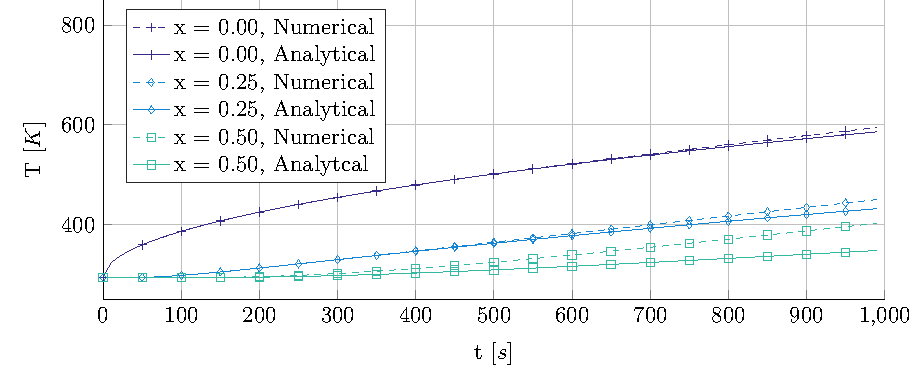
\includegraphics{Figure/Thermal/valcop.pdf}
	\caption[Comparison of analytical and numerical solution using a copper block]{Comparison of analytical and numerical solution by applying a constant heat flux for 1000 $\left[s\right]$ on a copper block with a 0.5 $\left[m\right]$ thickness.}
	\label{fig:valcop}
\end{figure}

\subsubsection{Validation against experimental data}
As mentioned earlier two papers by Del Corso et al provide the experimental data \cite{Corso2009,Corso2011}. The four lay-ups shown in Figure \ref{fig:vallayup} have been tested to validate the thermal model. Note that the references do not provide the experimental data for lay-up 1, but give the result of the thermal model they have used. For lay-up 2 and 3 data from both \gls{nasa}'s model and experiments have been provided. 


\begin{figure}[h]
	\centering
	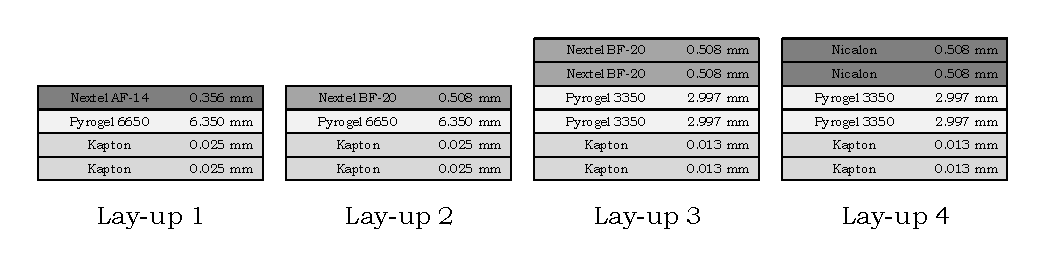
\includegraphics[width=\textwidth]{Figure/Thermal/vallayup.pdf}
	\caption{The four lay-ups used to test the thermal model against experimental data}
	\label{fig:vallayup}
\end{figure}

All lay-ups have been compared and validated. Before the model is validated all the contact resistances had to be adjusted such that they match the experimental data as was already mentioned in Section \ref{subsec:thermaltool}. The reason for this is that it is not possible to determine this value analytically. Lay-up 2 is used to serve as an example of this validation and has been subjected to a heat flux of 6.2 $\left[W\cdot cm^{-2}\right]$ for 90 $\left[s\right]$. Between every layer a thermocouple was placed during the experiment. With four layers that means that there were three thermocouples. Figure \ref{fig:plotvallay2} shows the result of this validation. It is clear that the model works very well during the application of the heat flux in the first 90 $\left[s\right]$. The average error for thermocouples TC1, TC2 and TC3 are 3.9 \%, 3.0 \% and 4.8 \% respectively. However, during the cooling down of the lay-up the error rapidly increases to 60.1 \%, 66.0 \% and 68.9 \%.

\begin{figure}[H]
	\centering
	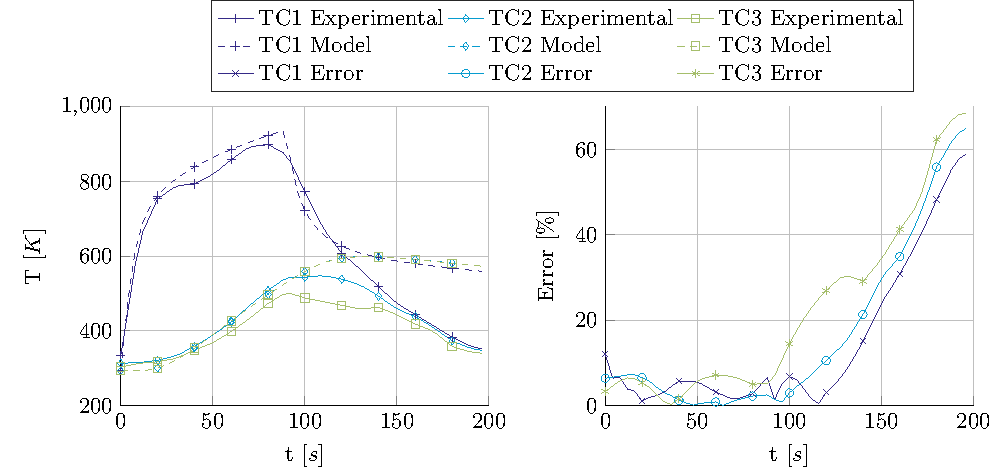
\includegraphics{Figure/Thermal/plotvallay2.pdf}
	\caption{Thermal model compared to experimental data at three locations}
	\label{fig:plotvallay2}
\end{figure}

Table \ref{tab:valerrorthermo} shows the result of all the lay-ups. The thermal model has been compared to \gls{nasa}'s model, the experimental data where possible. For reference NASA's model has been compared to the experimental data to show the performance of the developed thermal model. Note that the maximum error is the average of the maximum errors of the thermocouples. Also for every lay-up the contact resistance must be tweaked in order to match the experimental data. The number used in tweaking is characteristic for the two layers it seperates. The table shows that the thermal model is accurate to about 15-20 \%. \gls{nasa}'s model performs better with an accuracy of about 10-15 \%. Not visible in the table, but visible in Figure \ref{fig:plotvallay2} is that larger errors are overestimates of the temperatures. \textcolor{red}{BLABLABAL, layup 4 nog ingevuld worden}

\begin{table}[h]
	\centering
	\caption{Comparison of thermal model, \gls{nasa}'s model and experimental data}
	\begin{tabular}{|p{5.6cm}|rrrr|}
		\hline
		\textbf{} & \textbf{Lay-up 1} & \textbf{Lay-up 2} & \textbf{Lay-up 3} & \textbf{Lay-up 4} \\ \hline \hline
		\multicolumn{5}{|l|}{\textbf{Thermal model vs. experimental data}}			\\ \hline	
		Avg. error											&        - & 18.28 \% & 16.45 \% & 00.00 \% \\
		Max. error											&        - & 65.03 \% & 70.90 \% & 00.00 \% \\
		Avg. error during heat flux							&        - &  3.91 \% & 17.75 \% & 00.00 \% \\
		Avg. error during cooling down						&        - & 30.05 \% &  8.67 \% & 00.00 \% \\ \hline
		\multicolumn{5}{|l|}{\textbf{Thermal model vs. \gls{nasa}'s model}}			\\ \hline		
		Avg. error											&  6.72 \% & 10.88 \% & 17.85 \% & 00.00 \% \\
		Max. error											& 22.54 \% & 22.42 \% & 55.56 \% & 00.00 \% \\
		Avg. error during heat flux							&  7.26 \% & 10.48 \% & 18.19 \% & 00.00 \% \\
		Avg. error during cooling down						&  6.62 \% & 11.20 \% & 15.84 \% & 00.00 \% \\ \hline
		\multicolumn{5}{|l|}{\textbf{\gls{nasa}'s model vs. experimental data}}			\\ \hline		
		Avg. error											&        - & 13.79 \% & 10.69 \% & 00.00 \% \\
		Max. error											&        - & 43.37 \% & 34.22 \% & 00.00 \% \\
		Avg. error during heat flux							&        - &  8.43 \% & 10.28 \% & 00.00 \% \\
		Avg. error during cooling down						&        - & 18.18 \% & 13.15 \% & 00.00 \% \\ \hline
	\end{tabular}
	\label{tab:valerrorthermo}
\end{table}


\subsubsection{Conclusions after the verification and validation procedure}
The verification showed that the numerical solution starts to diverge as the error increases with time and depth. It is expected that this is a result of rounding errors that get multiplied every timestep in the discretisation scheme. The reason for this is that refining the mesh produces the same errors. There are two reasons why this is not a significant problem for the design problem. The first is that the \gls{tps} shall be a hundred times thinner. The second is that the length of the aerocapture and entry phases are approximately 400 $\left[s\right]$, which is lower than the 1000 $\left[s\right]$ in the verification. 
 
The validation shows that the thermal model, with an accuracy of 15-20 \%, performs slightly worse than \gls{nasa}'s model with an accuracy of 10-15 \%. Also the larger errors are overestimated temperatures, which makes designing with the model safe as it results in more conservative designs. It is assumed that errors under 10 \% should be completely acceptable for a low fidelity model. Larger error should be contributed to the difficulties in contact resistance modeling. When increasing the amount of layers it is increasingly difficult to predict the contact resistance, something Del Corso also experienced in \gls{nasa}'s model \cite{Corso2009}. This especially gets worse when there is no heat applied and the lay-up converges to an equilibrium state. For the purpose of the design of the lay-up for an inflatable heat shield this is not a problem, as the heat shield has enough time to cool down in the parking orbit after the aerocapture before it starts its final entry. For these reasons the thermal model is considered validated and safe to use for design while keeping its accuracy in mind.
\subsection{Control}

**Intro**

\subsubsection{Assumptions}

**Primary and Secondary assumptions**

\subsubsection{Trim point}

**Moment equilibrium figures/equations**
**CG-location plot(s)  with conclusion on CG for AoA~20 and sideslip angle=0**

\subsubsection{Stability}

**From E.Mooij**

\subsubsection{Available control systems}

**Intro**

\paragraph{\acrfull{cg} offset}

**Not nessesary for AoA, not feasible for sideslip**

\paragraph{Thrusters}

**Sebstiaan**

\paragraph{Aerodynamic surfaces}

**Guido**



